\chapter{Cas tests}


Dans ce chapitre nous illustrons quelques exemples sur l'exécution parallèle des flux du travail scientifiques.  



%Pour illustrer le ---- sur un cas concres 

\section{}

\subsection{ Opération de calcul }


On commence par un exemple simple pour valider la combinaison entre Chiron et Spoc. Il s'agit d'une opération d'addition entre les contenus des fichiers d'un format csv représentants des données tabulaires.


%une activité de l'opérateur Map. L'activité Ex3Act1 execute un extracteur extractor.cmd.  

cet exemple montre l'utilité de chiron d'automatiser des operations de calcul sur un grand nombre des fichiers .


%Les différents fichiers présents 


\begin{itemize}

\item {\bf La configuration des données}

Le fichier input.dataset organise le flux de données afin de le traiter par Chiron. C'est un fichier de format "csv". Il contient trois colonnes ID, FILE1, FILE2. L'identifiant ID indique un flux de travail à appliquer sur les champs suivants. Les champs FILE1 et FILE2 contiennent les chemins des fichiers des données à traiter. % On applique une opération d'addition sur les données de fichiers de FILE1 et FILE2. 


\item{Linvocation d'un programme SPOC }

Pour chaque activité existe un script qui fait le lien avec Chiron en invoquant le programme Spoc implémenté.


%pour Appliquer une opération d'addition entre deux colonnes des deux fichiers de format csv.


\item {la configuration de flux de travail}

Le fichier XML Chiron.xml, c'est le fichier de la configuration. Il est chargé d'exécuter une instance de flux de travail. De telle façon, il contien la description du comportement de chaque composantn dans un workflow conçu.

Input relation "iact1":

la relation iact1 est la relation d'entrée de l'activité act1. ID, FILE1, FILE2.

Output relation "oact1":

la relation oact1 est la relation produite par l'activité act1. ID, FILE1, FILE2, FILE3.

FILE3: un champ ajouté par l'extracteur présente la sortie de l'opération appliquer sur FILE1 et FILE2. 


\item {Add1$\_$Chiron$\_$vecteurs.byte}


Le programme de Spoc prend en arguments ID FILE1 FILE2. Il applique une opération d'addition entre la colonne V de fichier FILE1 et la colonne K de fichier FILE2, et met le résultat dans un fichier de sortie. Et Il ajoute dans la relation de sortie une colonne FILE3 qui contiennent les chemins de fichiers de sorties.





Dans la base de données, pour "File$\_$Workflow" on trouve deux tables Iact1 et Oact1.

La table iact1 contient les champs de la relation d'entrée.

La table oact1 contient les champs de la relation de sortie, on trouve la colonne FILE3 qui contient les chemins des fichiers de sorties.


\end{itemize}



\subsection{ Canny détection des contours } 


Dans cet exemple nous avons choisi d'appliquer le filtre de Canny. Nous avons opté ce choix car il illustre bien le flux de travail avec plusieurs activités qui s'enchaine d'une façon que la sortie d'une activité est une entré d'une autre.

Le filtre de Canny est utilisé en traitement d'images pour la détection des contours. L'entrée est une image en gris et la sortie est une image en noir et blanc avec une ligne blanche d'une largeur d'un pixel indiquant les bords. Un bord peut être défini comme un lieu de contraste élevé. 


L'algorithme de Canny est conçu pour être optimal suivant trois critères clairement explicités :

Bonne détection : faible taux d'erreur dans la signalisation des contours. Bonne localisation : minimisation des distances entre les contours détectés et les contours réels.

Clarté de la réponse : une seule réponse par contour et pas de faux positifs.%Sommaire

Il comporte quatre étapes: la réduction du bruit, le gradient d'intensité, la direction des contours, la suppression des non-maxima et le Seuillage des contours. Implimenter réspectivement par les filtres suivents flou gaussien, filtrage de sobel, suppression non maximale, le seuillage hystérésis.



On décrit ci-dessous brièvement chaque étape.

%1 Développement du filtre de Canny

\paragraph{flou gaussien }

%Mise en œuvre

Dans la première étape un flou gaussien est effectué pour réduire le bruit de l'image originale avant d'en détecter les contours. %Ceci permet d'éliminer les pixels isolés qui pourraient induire de faux réponses lors du calcul du gradient, conduisant ainsi à de faux positifs.

%Un filtrage gaussien 2D est utilisé ( Lissage de l'image), dont voici l'opérateur de convolution :

%et un exemple de masque 5×5 discret avec σ=1,4 :

%h = 1 159 [ 2 4 5 4 2 4 9 12 9 4 5 12 15 12 5 4 9 12 9 4 2 4 5 4 2 ] %%{\displaystyle h={\frac {1}{159}}{\begin{bmatrix}2&4&5&4&2\%\4&9&12&9&4\%\5&12&15&12&5\\4&9&12&9&4\\2&4&5&4&2\end{bmatrix}}} 

 Cela est nécessaire parce que le bruit est généralement un contraste élevé et conduirait donc à des faux positifs. Il est implémenté en utilisant la convolution de l'image. La convolution de l'image est une opération qui remplace essentiellement chaque pixel avec une moyenne pondérée de ses voisins. %Les poids choisis sont très importants et provoquent l'image convolution soit applicable à un certain nombre de problèmes. pixels Les poids de flou gaussien plus étroits plus lourdement que ceux éloignés.





 %L'opérateur utilisé permet de calculer le gradient suivant les directions X et Y, il est composé de deux masques de convolution, un de dimension 3,1 et l'autre 1,3. %G x = [ $/−$ 1 0 1 ] ; G y = [ 1 0 $/−$ 1 ]


% {\displaystyle G_{x}={\begin{bmatrix}-1&0&1\end{bmatrix}}\qquad ;\qquad G_{y}={\begin{bmatrix}1\\0\\-1\end{bmatrix}}} 


%La valeur du gradient en un point est approximée par la formule :


%| G | = | G x | + | G y | {\displaystyle |G|=|G_{x}|+|G_{y}|} 

\paragraph{Sobel filtre et direction des contours}

Après le filtrage, l'étape suivante est d'appliquer un gradient qui retourne l'intensité des contours. le filtrage de Sobel remplace chaque pixel par une dérivée de x et y d'une combination des pixels voisins. Ce faisant, les pixels dans les zones de contraste élevé seront plus brillant que les pixels dans les zones de contraste faible. Ceci trouve essentiellement les zones où les bords sont plus susceptibles d'exister, mais il ne repérer pas précisément où les bords sont. Comme pour le flou gaussien, cela se fait en utilisant l'image convolution, mais la convolution est effectuée sur deux fois: une fois pour le dérivé de x et une fois pour le dérivé de y. Le pixel est alors remplacé par l'essentiel:% sqrt ((di / dx) ^ 2 + (di / dy) ^ 2) 

 où di représente le changement d'intensité. Au cours de cette étape, la direction du gradient est également calculé pour chaque pixel qui est nécessaire pour une suppression non maximale. Les orientations des contours sont déterminées par la formule :

%θ = ± arctan ⁡ ( G y G x ) {\displaystyle \theta =\pm \arctan \left({\frac {G_{y}}{G_{x}}}\right)} 

Nous obtenons finalement une carte des gradients d'intensité en chaque point de l'image accompagnée des directions des contours.



\paragraph{Suppression des non-maximum}


La carte des gradients obtenue précédemment fournit une intensité en chaque point de l'image. Une forte intensité indique une forte probabilité de présence d'un contour. Toutefois, cette intensité ne suffit pas à décider si un point correspond à un contour ou non. Seuls les points correspondant à des maxima locaux sont considérés comme correspondant à des contours, et sont conservés pour la prochaine étape de la détection. Un maximum local est présent sur les extrema du gradient, c'est-à-dire là où sa dérivée s'annule.


%À ce stade, il existe des gradients représentant des bords probables, mais notre objectif final est de représenter les bords comme une seule ligne de 1 pixel. 

suppression non maximale exclut les pixels qui font partie d'un bord, mais ne définissent pas le bord. Le résultat est que nous condensons ces bords de gradient de large en une seule ligne de 1 pixel. Notez que le résultat produit est toujours pas le produit fini, ces lignes ne sont pas purement blanc et ne signifient pas nécessairement un avantage, ils représentent encore la place une probabilité d'un bord. la suppression de non-maximale est effectuée en utilisant la direction du gradient trouvé à l'étape précédente et en comparant le pixel courant avec des pixels voisins de chaque côté. Si le pixel est plus faible en intensité que l'éther de ces pixels voisins, alors il est pas considéré être le bord vrai, si sa valeur est remplacée par 0. Si le pixel est la plus forte intensité de ses voisins dans la direction du gradient, puis il peut être le bord vrai, si sa valeur est conservée.


\paragraph{Seuillage des contours}


La différenciation des contours sur la carte générée se fait par seuillage à hysteresis. Cela nécessite deux seuils, un haut et un bas; qui seront comparés à l'intensité du gradient de chaque point. Le critère de décision est le suivant. Pour chaque point, si l'intensité de son gradient est inférieur au seuil bas, le point est rejeté, et si il est supérieur au seuil haut, le point est accepté comme formant un contour. Entre le seuil bas et le seuil haut, le point est accepté s'il est connecté à un point déjà accepté. Une fois ceci réalisé, l'image obtenue est binaire avec d'un côté les pixels appartenant aux contours et les autres.


ci desous l'implémentation de l'algorithme de Canny détection de bord en utilisant CHIRON et Spoc.


\paragraph{Le flux de travail}


On présise la structure de flux de travail dans le fichier XML. Le workflow est constituées de 5 taches, chaque tache correspond à un filtre.

%ous avons maintenant 1 pixel de largeur des lignes avec des valeurs indiquant la force du bord. Afin de décider lequel de ces devrait être considéré comme un avantage, nous allons utiliser deux valeurs de seuil. Le seuil bas indique que les pixels de moins que sa valeur ne peut pas être bords. Le seuil haut indique que les pixels supérieurs à sa valeur doivent être bords. Pixels entre ces valeurs ne seront bords si elles voisin d'un bord. Le seuil bas peut donc être considérée comme affectant la longueur des bords et le seuil haut peut être considéré comme affectant le nombre d'arêtes. En raison de la définition, la sortie correcte de ce stade ne peut pas être trouvé dans une seule passe l'examen pixels seulement voisins, car un "peut-être" bord peut aller de toute façon. Cela dit, une approximation peut être faite qui donne des performances considérablement augmenté (puisque aucun bord traversal est nécessaire) tout en conservant la précision de sortie suffisamment élevée pour la plupart des applications. Cette implémentation utilise l'approche d'approximation.






%Paramètres

%Les deux paramètres principaux déterminant le temps de calcul et l'acuité de l'algorithme sont la taille du filtre gaussien et les deux seuils.

%Taille du filtre: le filtre utilisé lors de la réduction du bruit a une influence directe sur le comportement de l'algorithme. Un filtre de petite taille produit un effet de flou moins prononcé, ce qui permet la détection de petites lignes bien marquées. Un filtre de taille plus grande produit un effet de flou plus important, ce qui permet de détecter des contours moins nets, par exemple celui d'un arc-en-ciel.


%Seuils: l'utilisation de deux seuils au lieu d'un améliore la flexibilité mais certains problèmes propres au seuillage demeurent. Ainsi, un seuil trop bas peut conduire à la détection de faux positifs. Inversement, un seuil trop haut peut empêcher la détection de contours peu marqués mais représentant de l'information utile.


%Il n'existe pas actuellement de méthode générique pour déterminer des seuils produisant des résultats satisfaisants sur tous les types d'images.




%\subsection{}



%Méthodes d'optimisation Dans un premier temps, un seul ensemble de noyaux OpenCL ont été utilisés qui ont été conçu pour fonctionner à la fois sur le CPU et le GPU. La performance sur le CPU était meilleur que prévu; il a donné 7x speedups plus de série sur un processeur quatre coeur. Cependant, les performances du GPU était beaucoup plus faible que prévu; il était plus lent que série. Le problème a été mis en évidence redondants mémoire globale accède. Parce que la plupart des étapes exigent que chaque pixel ont connaissance des pixels voisins, chaque pixel a été récupéré 9 fois ou plus de mémoire globale. Ce modèle d'accès est précisément ce que les GPU sont faibles à, beaucoup de ce qui aurait dû être exécuté en parallèle était en cours sérialisé par la mémoire globale des accès.



%Pour résoudre ce problème, deux groupes de travail dimensionnelles ont été utilisés. Chaque donnée de groupe de travail copies de pixels à la mémoire locale qui est beaucoup plus rapide, mais seulement accessible à partir de l'intérieur de ce groupe de travail. Cette mémoire globale réduite accède de manière significative et a donné un speedup 29x sur la version précédente. Le résultat final était 8-13x accélération sur série pour le GPU, avec des performances de pointe pour les images qui sont d'environ 10 millions de pixels. Lors de l'exécution sur la CPU, cette mise en œuvre a eu une accélération 7-10x sur les images entre 0.3-9 mégapixels, mais est tombé très rapidement pour les grandes images.

\begin {table}[!h]
\centering
\begin{tabular} {|p{2cm}|p{2cm}|p{2cm}|p{2cm}||p{3cm}|}

  \hline

 & filtre & input & output &  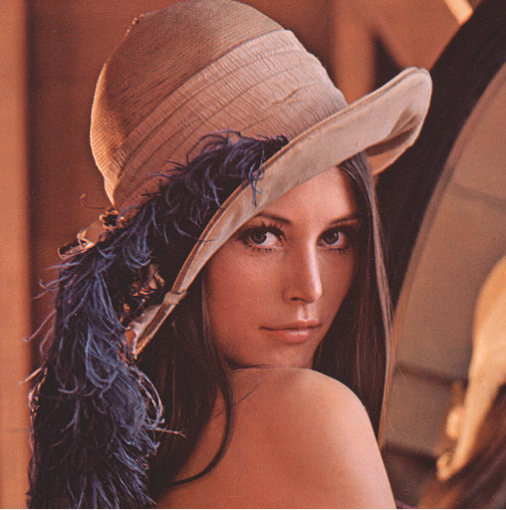
\includegraphics[width=3cm, height=3cm]{images/lena.png}\\\\

  \hline

 act1 &  gray  & image & oact1& 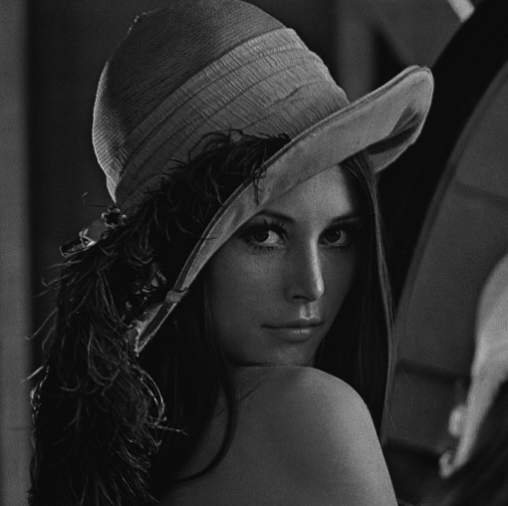
\includegraphics[width=3cm, height=3cm]{images/1.png}\\

   \hline

  act2 & Gaussian & image1 & image2 & 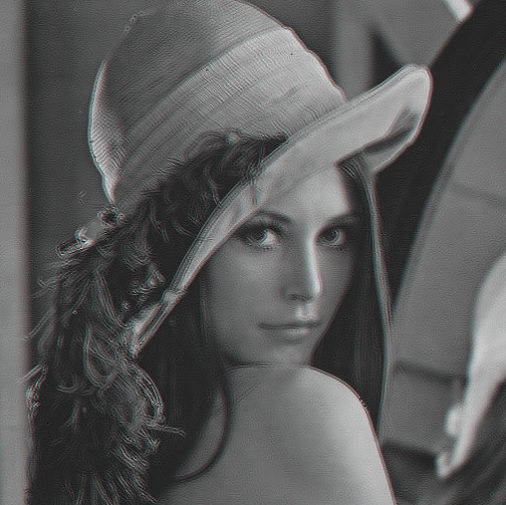
\includegraphics[width=3cm, height=3cm]{images/2.png}\\

  \hline

    act3 & Sobel & 2.3 & image3 & 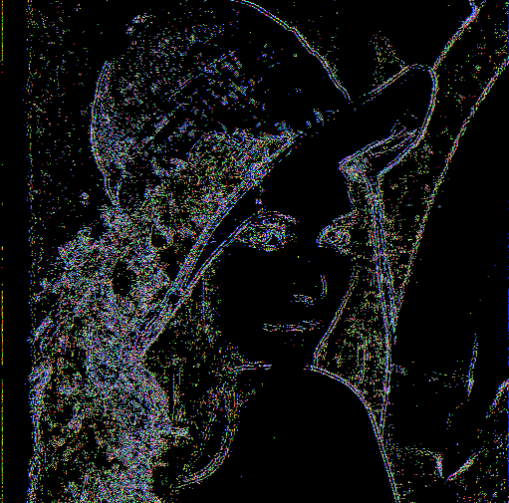
\includegraphics[width=3cm, height=3cm]{images/3.png}\\

  \hline

    act4 & Non-max & image3  & image4 &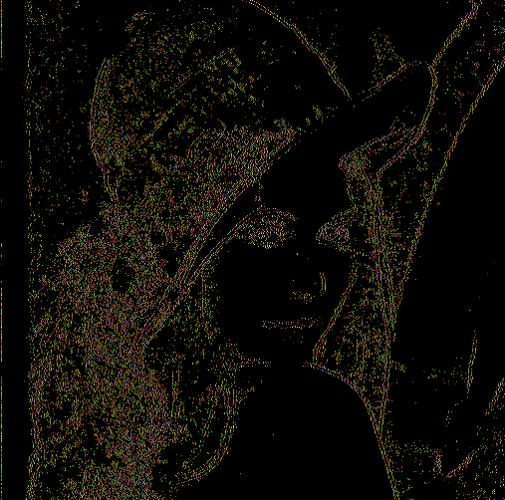
\includegraphics[width=3cm, height=3cm]{images/4.png} \\

  \hline

    act5 & hysteris & mage4 & image5 & 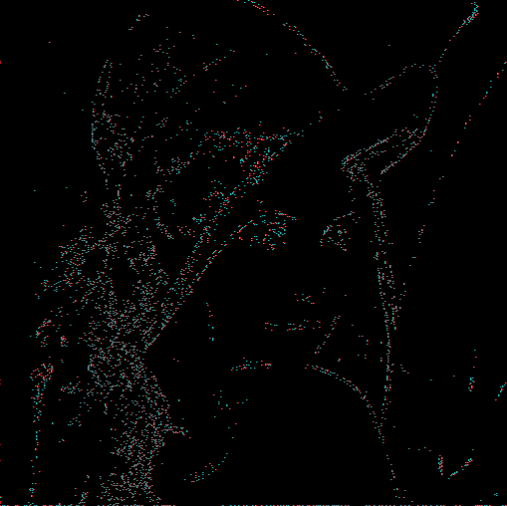
\includegraphics[width=3cm, height=3cm]{images/5.png}\\

  \hline

\end{tabular}
\caption{Le flux de travail de canny}
\end{table}
